%\documentclass[handout]{beamer}
\documentclass[t,12pt,numbers,fleqn]{beamer}
%\documentclass[ignorenonframetext]{beamer}

\newif\ifquestions
%\questionstrue
\questionsfalse

\usepackage{pgfpages}
\usepackage{hyperref}
\hypersetup{colorlinks=true,
    linkcolor=blue,
    citecolor=blue,
    filecolor=blue,
    urlcolor=blue,
    unicode=false}
\urlstyle{same}

\usepackage{booktabs}

\usepackage{caption}
\usepackage{subcaption}
\captionsetup[figure]{font=scriptsize,labelfont=scriptsize}

\usepackage[version=4]{mhchem}
\usepackage{siunitx}
\usepackage{tabularx}

%% Common Parts

\newcommand{\progname}{MPIR} % PUT YOUR PROGRAM NAME HERE
\newcommand{\authname}{Xunzhou (Joe) Ye} % AUTHOR NAMES

\newcommand{\matr}[1]{\mathbf{#1}}
\renewcommand{\vec}[1]{\mathbf{#1}}

\usepackage{hyperref}
    \hypersetup{colorlinks=true, linkcolor=blue, citecolor=blue, filecolor=blue,
                urlcolor=blue, unicode=false}
    \urlstyle{same}


%\usetheme{Iimenau}

\useoutertheme{split} %so the footline can be seen, without needing pgfpages

%\pgfpagesuselayout{resize to}[letterpaper,border shrink=5mm,landscape]  %if this is uncommented, the hyperref links do not work

\mode<presentation>{}

%% Requires:
%%
%% \usepackage{latexsym}
%% \usepackage{amssymb}
%% \usepackage{stmaryrd}

%\renewcommand{\labelenumi}{(\theenumi)}

\newcommand{\be}{\begin{enumerate}}
\newcommand{\ee}{\end{enumerate}}
\newcommand{\bi}{\begin{itemize}}
\newcommand{\ei}{\end{itemize}}
\newcommand{\bc}{\begin{center}}
\newcommand{\ec}{\end{center}}
\newcommand{\bsp}{\begin{sloppypar}}
\newcommand{\esp}{\end{sloppypar}}

\newcommand{\sglsp}{\ }
\newcommand{\dblsp}{\ \ }

\newcommand{\iclicker}{i\texttt{>}clicker}

\newcommand{\sA}{\mbox{$\cal A$}}
\newcommand{\sB}{\mbox{$\cal B$}}
\newcommand{\sC}{\mbox{$\cal C$}}
\newcommand{\sD}{\mbox{$\cal D$}}
\newcommand{\sE}{\mbox{$\cal E$}}
\newcommand{\sF}{\mbox{$\cal F$}}
\newcommand{\sG}{\mbox{$\cal G$}}
\newcommand{\sH}{\mbox{$\cal H$}}
\newcommand{\sI}{\mbox{$\cal I$}}
\newcommand{\sJ}{\mbox{$\cal J$}}
\newcommand{\sK}{\mbox{$\cal K$}}
\newcommand{\sL}{\mbox{$\cal L$}}
\newcommand{\sM}{\mbox{$\cal M$}}
\newcommand{\sN}{\mbox{$\cal N$}}
\newcommand{\sO}{\mbox{$\cal O$}}
\newcommand{\sP}{\mbox{$\cal P$}}
\newcommand{\sQ}{\mbox{$\cal Q$}}
\newcommand{\sR}{\mbox{$\cal R$}}
\newcommand{\sS}{\mbox{$\cal S$}}
\newcommand{\sT}{\mbox{$\cal T$}}
\newcommand{\sU}{\mbox{$\cal U$}}
\newcommand{\sV}{\mbox{$\cal V$}}
\newcommand{\sW}{\mbox{$\cal W$}}
\newcommand{\sX}{\mbox{$\cal X$}}
\newcommand{\sY}{\mbox{$\cal Y$}}
\newcommand{\sZ}{\mbox{$\cal Z$}}

\renewcommand{\phi}{\varphi}
\newcommand{\seq}[1]{{\langle #1 \rangle}}
\newcommand{\set}[1]{{\{ #1 \}}}
\newcommand{\tuple}[1]{{( #1 )}}
\newcommand{\mlist}[1]{{[ #1 ]}}
\newcommand{\sembrack}[1]{\llbracket#1\rrbracket}
%\newcommand{\sembrack}[1]{[\![#1]\!]}
\newcommand{\synbrack}[1]{\ulcorner#1\urcorner}
\newcommand{\commabrack}[1]{\lfloor#1\rfloor}
\newcommand{\bsynbrack}[1]{\lceil#1\rceil}
\newcommand{\bsembrack}[1]{\lceil\!\!\lceil#1\rceil\!\!\rceil}
\newcommand{\mname}[1]{\mbox{\sf #1}}
\newcommand{\mcolon}{\mathrel:}
\newcommand{\mdot}{\mathrel.}
\newcommand{\modpar}{\models_{\rm par}}
\newcommand{\modreg}{\models_{\rm reg}}
\newcommand{\proves}[2]{#1 \vdash #2}
\newcommand{\notproves}[2]{#1 \not\vdash #2}
\newcommand{\provesin}[3]{#1 \vdash_{#2} #3}
\newcommand{\notprovesin}[3]{#1 \not\vdash_{#2} #3}
%\newcommand{\leqq}[1]{\mathrel{\preceq_{#1}}}
\newcommand{\parrow}{\rightharpoonup}
\newcommand{\tarrow}{\rightarrow}
\newcommand{\term}{\seq}
\newcommand{\lub}{\sqcup}
\newcommand{\subfun}{\sqsubseteq}
\newcommand{\subpred}{\subseteq}
\newcommand{\BoxApp}{\Box\,}
\newcommand{\BOX}{\mathrel{\Box}}
\newcommand{\funapp}{\mathrel@}

\newcommand{\com}{\mname{complement}}
\newcommand{\dom}{\mname{domain}}
\newcommand{\sumcl}{\mname{sum}}
\newcommand{\pow}{\mname{power}}
\newcommand{\pair}{\mname{pair}}
\newcommand{\opair}{\mname{ordered-pair}}
\newcommand{\inters}{\mname{intersection}}
\newcommand{\emp}{\mname{empty}}
\newcommand{\uni}{\mname{univocal}}
\newcommand{\fun}{\mname{function}}
\newcommand{\card}{\mname{card}}
\newcommand{\sets}{\mname{sets}}
\newcommand{\monotone}{\mname{monotone}}
\newcommand{\continuous}{\mname{continuous}}
\newcommand{\chain}{\mname{chain}}
\newcommand{\mub}{\mname{ub}}
\newcommand{\mlub}{\mname{lub}}
\newcommand{\fixedpoint}{\mname{fp}}
\newcommand{\leastfixedpoint}{\mname{lfp}}
\newcommand{\strongfixedpoint}{\mname{sfp}}
\newcommand{\emptyfun}{\triangle}
\newcommand{\statetrans}[1]{\stackrel{#1}{\longrightarrow}}
\newcommand{\thyext}{\leq}
\newcommand{\conthyext}{\unlhd}

\newcommand{\Iota}{\mbox{\rm I}}
\newcommand{\IotaApp}{\mbox{\rm I}\,}
\newcommand{\iotaApp}{\iota\,}
\newcommand{\epsilonApp}{\epsilon\,}
\newcommand{\True}{\mbox{\sf T}}
\newcommand{\False}{\mbox{\sf F}}
\newcommand{\Trueword}{\sf true}
\newcommand{\Falseword}{\sf false}
\newcommand{\Neg}{\neg}
\newcommand{\Andd}{\wedge}
\newcommand{\Or}{\vee}
\newcommand{\Implies}{\supset}
\newcommand{\ImpliesAlt}{\Rightarrow}
\newcommand{\Iff}{\equiv}
\newcommand{\Sheffer}{\mathrel|}
\newcommand{\IffAlt}{\Leftrightarrow}
\newcommand{\Forall}{\forall}
\newcommand{\ForallApp}{\forall\,}
\newcommand{\Forsome}{\exists}
\newcommand{\ForsomeApp}{\exists\,}
\newcommand{\ForsomeUniqueApp}{\exists\,!\,}
\newcommand{\IsDef}{\downarrow}
\newcommand{\IsUndef}{\uparrow}
\newcommand{\Equal}{=}
\newcommand{\QuasiEqual}{\simeq}
\newcommand{\Undefined}{\bot}
\newcommand{\If}{\mname{if}}
\newcommand{\IsDefApp}{\!\IsDef}
\newcommand{\IsUndefApp}{\!\IsUndef}
\newcommand{\TRUE}{\mbox{{\sc t}}}
\newcommand{\FALSE}{\mbox{{\sc f}}}
\newcommand{\truthvalues}{\{\TRUE,\FALSE\}}
\newcommand{\LambdaApp}{\lambda\,}
\newcommand{\LAMBDAapp}{\Lambda\,}
\newcommand{\AlphaEquiv}{\stackrel{\alpha}{=}}

\newcommand{\mvar}[3]{\textbf{var}_{#1}[#2,#3]}
\newcommand{\mterm}[2]{\textbf{term}_{#1}[#2]}
\newcommand{\mform}[2]{\textbf{form}_{#1}[#2]}
\newcommand{\mtype}[2]{\textbf{type}_{#1}[#2]}
\newcommand{\mexpr}[3]{\textbf{expr}_{#1}[#2,#3]}

\newcommand{\imps}{\mbox{\sc imps}}
\newcommand{\fol}{\mbox{\sc fol}}
\newcommand{\lutins}{\mbox{\sc lutins}}
\newcommand{\vlisp}{\mbox{\sc vlisp}}
\newcommand{\vmach}{\mbox{\sc vmach}}
\newcommand{\gnu}{\mbox{\sc gnu}}
\newcommand{\zf}{\mbox{\sc zf}}
\newcommand{\nbg}{\mbox{\sc nbg}}
\newcommand{\pnbg}{\mbox{\sc pnbg}}
\newcommand{\snbg}{\mbox{\sc snbg}}
\newcommand{\pfol}{\mbox{\sc pfol}}
\newcommand{\nbgstar}{$\mbox{\sc nbg}^\ast$}
\newcommand{\boldnbgstar}{$\mbox{\bf NBG}^\ast$}
\newcommand{\stt}{\mbox{\sc stt}}
\newcommand{\eves}{\mbox{\sc eves}}
\newcommand{\hol}{\mbox{\sc hol}}
\newcommand{\mizar}{Mizar}
\newcommand{\nqthm}{Nqthm}
\newcommand{\pvs}{\mbox{\sc pvs}}
\newcommand{\stmm}{\mbox{\sc stmm}}

\iffalse
\newtheorem{thm}{Theorem}[section]
\newtheorem{cor}[thm]{Corollary}
\newtheorem{lem}[thm]{Lemma}
\newtheorem{prop}[thm]{Proposition}
\newtheorem{rem}[thm]{Remark}
\newtheorem{eg}[thm]{Example}
\newtheorem{df}[thm]{Definition}
\fi

%\newenvironment{proof}{\par\noindent{\bf Proof\ \ }}{$\Box$}

\newenvironment{namedform}[1]
   {\begin{tabbing}\textbf{#1}\ }
   {\end{tabbing}}

\newcommand{\urlpart}[1]{\mbox{\texttt{#1}}\linebreak[0]}

\newcommand{\bblue}{\textcolor{blue!80!black}}
\newcommand{\bgreen}{\textcolor{green!55!black}}
\newcommand{\bbrown}{\textcolor{brown}}
\newcommand{\bred}{\textcolor{red!80!black}}
\newcommand{\bcyan}{\textcolor{cyan!80!black}}
\newcommand{\bmagenta}{\textcolor{magenta}}
\newcommand{\byellow}{\textcolor{yellow}}
\newcommand{\borange}{\textcolor{orange}}
\newcommand{\bviolet}{\textcolor{violet}}
\newcommand{\bpurple}{\textcolor{purple}}
\newcommand{\bdarkgray}{\textcolor{darkgray}}
\newcommand{\bgray}{\textcolor{gray}}
\newcommand{\blightgray}{\textcolor{lightgray}}

\newcommand{\clicker}{i\texttt{>}clicker}

\newenvironment{changemargin}[2]{%
  \begin{list}{}{%
    \setlength{\topsep}{0pt}%
    \setlength{\leftmargin}{#1}%
    \setlength{\rightmargin}{#2}%
    \setlength{\listparindent}{\parindent}%
    \setlength{\itemindent}{\parindent}%
    \setlength{\parsep}{\parskip}%
  }%
  \item[]}{\end{list}}


\newcommand{\topic}{Mixed-Precision Iterative Solver}

%Title page information for 1D04 lectures slides

% Define year specific parameters - used in title page and footer

\newcommand{\season}{Winter} %use to switch between Winter and Fall
\newcommand{\instructor}{Xunzhou (Joe) Ye} %use to switch instructor
\newcommand{\instructSmall}{Xunzhou}
\newcommand{\yr}{2025}
\newcommand{\courseCode}{CAS 741}
\newcommand{\courseTitle}{Development of Scientific Computing Software}

%\setbeamerfont{structure}{series=\bfseries}
%\usefonttheme[stillsansseriftext,stillsansserifmath]{serif}
\setbeamertemplate{navigation symbols}{}
\setbeamertemplate{itemize item}[ball]

\title{
  {\normalsize \bf
    \borange{\courseCode~(\courseTitle)\\ \season~\yr}}\\[2ex]
  {\Large \bf \topic}}

\author[Smith]{\instructor}

\institute{
  Faculty of Engineering,
  McMaster University}

\date{
\today
\bc
  
\includegraphics[scale = 0.2, keepaspectratio]
  {../../mcmaster-logo-full-color.jpg}
\ec
}

\renewcommand{\borange}[1] %orange is too hard to read
{
   \bred{#1}
}


\begin{document}

% Footline for  Slides

% Display title page and displays footers

\setbeamertemplate{footline}{} %so the title screen does not have a footline

%%%%%%%%%%%%%%%%%%%%%%%%%%%%%%%%%%%%%%%%%%%%%%%%%%%%%%%%%%%%

\begin{frame}
\titlepage
\end{frame}

%%%%%%%%%%%%%%%%%%%%%%%%%%%%%%%%%%%%%%%%%%%%%%%%%%%%%%

\setbeamertemplate{footline}{
\begin{beamercolorbox}{sectioninhead/foot}
\hspace{1ex}\bblue{\hrulefill}\hspace{1ex}

\vspace{1ex}
\hspace{1ex}
{\tiny \instructSmall \hfill
\courseCode~\season~\yr:~\topic \hfill
\insertframenumber/\inserttotalframenumber~~}
%\insertframenumber/\ref{lastframe}}
%\hfill {\small \insertframenumber} \hspace{10ex}
%{\small $$\insertframenumber$$}
\vspace{1ex}
\end{beamercolorbox}}

%%%%%%%%%%%%%%%%%%%%%%%%%%%%%%%%%%%%%%%%%%%%%%%%%%%%%%


%%%%%%%%%%%%%%%%%%%%%%%%%%%%%%%%%%%%%%%%%%%%%%%%%%%%%%

\begin{frame}
\frametitle{Linear Solver: the Good Old \(\matr{A}\vec{x} = \vec{b}\) Problem}

\begin{itemize}
\item Direct method: Gaussian elimination
\end{itemize}

\[
  \begin{aligned}
    \matr{A}\vec{x} = &
    \left[
    \begin{array}{ccc}
      1 & -1 & 3 \\
      1 &  1 & 0 \\
      3 & -2 & 1
    \end{array}
    \right]
    \begin{bmatrix}
      x_1 \\
      x_2 \\
      x_3
    \end{bmatrix}
    =
    \begin{bmatrix}
      11 \\
      3 \\
      3
    \end{bmatrix}
    = \vec{b}
    \\
    \matr{A}|\vec{b} = &
    \left[
    \begin{array}{ccc|c}
      1 & -1 & 3 & 11 \\
      1 &  1 & 0 &  3 \\
      3 & -2 & 1 &  3
    \end{array}
    \right]
    \begin{array}{cc}
      \times 1 & \times 3 \\
      \downarrow   & \\
               & \downarrow
    \end{array}
    \\
    \matr{A}|\vec{b} \leftarrow &
    \left[
    \begin{array}{ccc|c}
      1 & -1 & 3 &  11 \\
      0 &  2 & -3 &  -8 \\
      0 &  1 & -8 & -30
    \end{array}
    \right]
  \end{aligned}
\]

\end{frame}

%%%%%%%%%%%%%%%%%%%%%%%%%%%%%%%%%%%%%%%%%%%%%%%%%%%%%%%%%%%%%%%%%%%%%%%%%%%%%

\begin{frame}
\frametitle{Think Big, Think Sparse}

\begin{itemize}
\item In structural simulations (e.g., finite element analysis), structures are
  modeled based on real-world physics, where forces and constraints are often
  localized.
\item Each element or node in a structure is typically connected only to a few
  nearby elements or nodes.
\item System of equations in structural simulations is assembled from local
  contributions.
\item In contrast, in neural networks, dense weight matrices are used in fully
  connected layers.
\end{itemize}

\end{frame}

%%%%%%%%%%%%%%%%%%%%%%%%%%%%%%%%%%%%%%%%%%%%%%%%%%%%%%%%%%%%%%%%%%%%%%%%%%%%%

\begin{frame}
\frametitle{Sparse Matrix Example: Boeing/ct20stif}

\begin{itemize}
\item \(\num{52329} \times \num{52329}\)
\item \num{2600295} non-zeros
\item \(\approx \SI{33}{\mega\byte}\) in file size
\end{itemize}

\begin{figure}[h]
  \centering
  \begin{subfigure}[b]{0.5\textwidth}
    \centering
    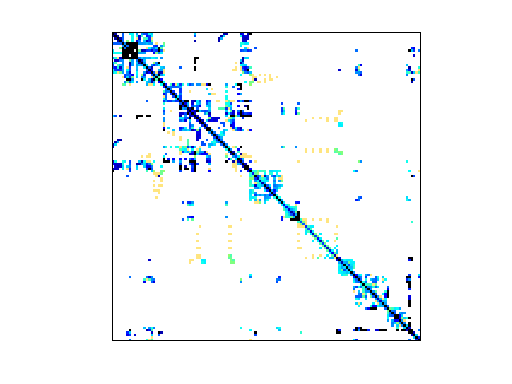
\includegraphics[width=\textwidth,trim={2cm 1.5cm 2cm 1cm},clip]{figures/ct20stif}
  \end{subfigure}
  \begin{subfigure}[b]{0.4\textwidth}
    \centering
    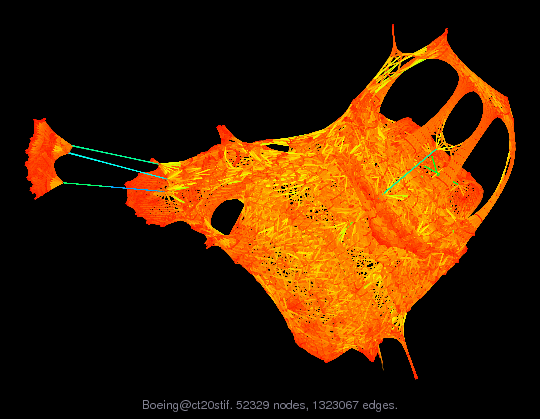
\includegraphics[width=\textwidth]{figures/ct20stif_graph}
  \end{subfigure}
  \caption*{Boeing/ct20stif: CT20 Engine Block -- Stiffness
    matrix}
  \label{fig:ct20}
\end{figure}

\end{frame}

%%%%%%%%%%%%%%%%%%%%%%%%%%%%%%%%%%%%%%%%%%%%%%%%%%%%%%%%%%%%%%%%%%%%%%%%%%%%%

\begin{frame}
\frametitle{Sparse Matrix Example: Janna/Serena}

\begin{itemize}
\item \(\num{1391349} \times \num{1391349}\)
\item \num{64131971} non-zeros
\item \(\approx \SI{847}{\mega\byte}\) in file size
\end{itemize}

\begin{figure}[hh]
  \centering
  \begin{subfigure}[b]{0.5\textwidth}
    \centering
    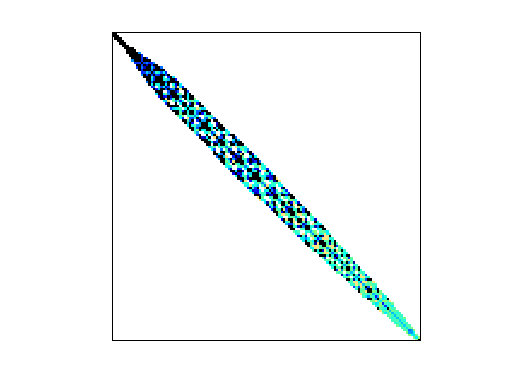
\includegraphics[width=\textwidth,trim={2cm 1.5cm 2cm 1cm},clip]{figures/Serena}
  \end{subfigure}
  \begin{subfigure}[b]{0.37\textwidth}
    \centering
    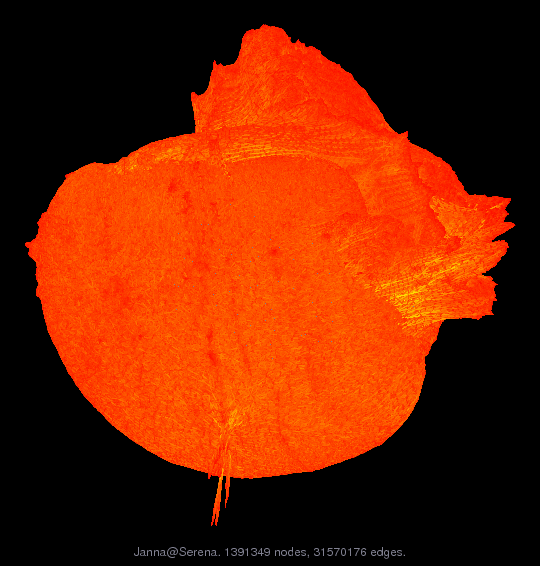
\includegraphics[width=\textwidth]{figures/Serena_graph}
  \end{subfigure}
  \caption*{Janna/Serena: gas resevoir simulation for \ce{CO2}
    sequestration}
  \label{fig:Serena}
\end{figure}

\end{frame}

%%%%%%%%%%%%%%%%%%%%%%%%%%%%%%%%%%%%%%%%%%%%%%%%%%%%%%%%%%%%%%%%%%%%%%%%%%%%%

\begin{frame}
\frametitle{The Problem with Gaussian Elimination}

\begin{itemize}
\item Store the whole matrix
\item Memory bounded
\end{itemize}

\[
  \begin{aligned}
    \matr{A}|\vec{b} = &
    \left[
      \begin{array}{ccc|c}
        1 & -1 & 3 & 11 \\
        1 &  1 & 0 &  3 \\
        3 & -2 & 1 &  3
      \end{array}
    \right]
    \begin{array}{cc}
      \times 1 & \times 3 \\
      \downarrow   & \\
               & \downarrow
    \end{array}
    \\
    \matr{A}|\vec{b} \leftarrow &
    \left[
    \begin{array}{ccc|c}
      1 & -1 & 3 &  11 \\
      0 &  2 & -3 &  -8 \\
      0 &  1 & -8 & -30
    \end{array}
    \right]
  \end{aligned}
\]

\end{frame}

%%%%%%%%%%%%%%%%%%%%%%%%%%%%%%%%%%%%%%%%%%%%%%%%%%%%%%%%%%%%%%%%%%%%%%%%%%%%%

\begin{frame}
\frametitle{The Problem with Gaussian Elimination}

\begin{itemize}
\item Sparsity preservation
\end{itemize}

\begin{figure}[h]
  \centering
  \begin{subfigure}[b]{0.5\textwidth}
    \centering
    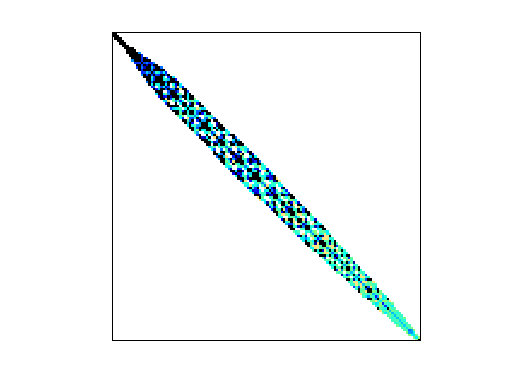
\includegraphics[width=\textwidth,trim={2cm 1.5cm 2cm 1cm},clip]{figures/Serena}
  \end{subfigure}
  \begin{subfigure}[b]{0.37\textwidth}
    \centering
    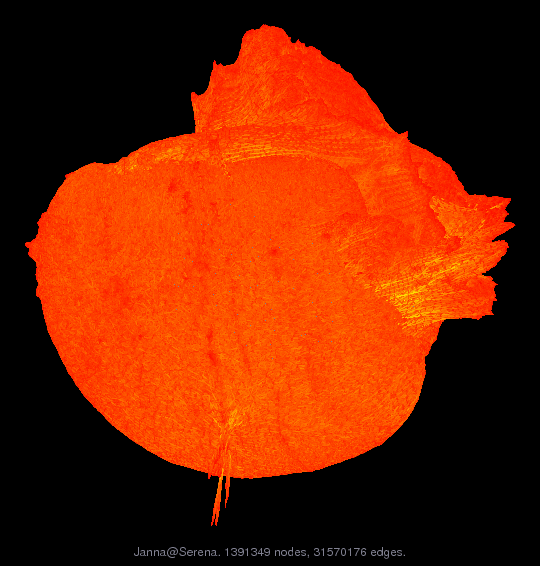
\includegraphics[width=\textwidth]{figures/Serena_graph}
  \end{subfigure}
  \caption*{Janna/Serena: gas resevoir simulation for \ce{CO2}
    sequestration}
  \label{fig:Serena}
\end{figure}

\end{frame}

%%%%%%%%%%%%%%%%%%%%%%%%%%%%%%%%%%%%%%%%%%%%%%%%%%%%%%%%%%%%%%%%%%%%%%%%%%%%%

\begin{frame}
\frametitle{Iterative Refinement}

\begin{itemize}
\item A method to enhance the accuracy of a solution to \(\matr{A}\vec{x} = \vec{b}\)
\end{itemize}

The algorithm goes:
\begin{enumerate}
\item Solve \(\matr{A}\vec{x}_0 = \vec{b}\) \emph{approximately} to get an initial solution \(\vec{x}_0\).
\item Compute the residual \(\vec{r} = \vec{b} - \matr{A}\vec{x}_0\), which measures how far \(\vec{x}_0\) is
  from being an exact solution.
\item Solve \(\matr{A}\vec{e} = \vec{r}\) for the correction vector \(\vec{e}\).
\item Update (``refine'') the solution as \(\vec{x}_1 = \vec{x}_0 + \vec{e}\).
\item Repeat steps 2--4 until the residual \(\vec{r}\) is small enough.
\end{enumerate}

\end{frame}

%%%%%%%%%%%%%%%%%%%%%%%%%%%%%%%%%%%%%%%%%%%%%%%%%%%%%%%%%%%%%%%%%%%%%%%%%%%%%

\begin{frame}
\frametitle{Iterative Refinement in Mixed-Precision}

\begin{enumerate}
\item Solve \(\matr{A}\vec{x}_0 = \vec{b}\) \emph{approximately} in \textbf{low} precision.
\item Compute the residual \(\vec{r} = \vec{b} - \matr{A}\vec{x}_0\) in \textbf{high} precision.
\item Solve \(\matr{A}\vec{e} = \vec{r}\) for the correction vector \(\vec{e}\) in \textbf{low} precision.
\item Update the solution as \(\vec{x}_1 = \vec{x}_0 + \vec{e}\) in \textbf{medium} precision.
\item Repeat steps 2--4 until the residual \(\vec{r}\) is small enough.
\end{enumerate}

Key points:

\begin{itemize}
\item Trade computational complexity for space complexity
\item Choose algorithms that can preserve sparsity: sparse LU factorization,
  General Minimal Residual Method (GMRES)
\item Inner solves could also be iterative and in mixed-precision
\item Possible matrix-free implementation
\end{itemize}

\end{frame}

%%%%%%%%%%%%%%%%%%%%%%%%%%%%%%%%%%%%%%%%%%%%%%%%%%%%%%%%%%%%%%%%%%%%%%%%%%%%%

\begin{frame}
\frametitle{Goals}

\begin{enumerate}[{GS}1]
\item Given some matrix \(\matr{A}\) and column vector \(\vec{b}\), the solver
  should iteratively find \(\vec{x}\) satisfying the equation \(\matr{A}\vec{x}
  = \vec{b}\) until the norm of the residual \(\vec{r} = \matr{A}\vec{x} -
  \vec{b}\) is smaller than some tolerance \(\epsilon\), or the maximum number
  of iterations \(n_\mathrm{iter}\) is exhausted, whichever comes first.
\item Given some combinations of floating point precision configuration, the solver
  should perform internal steps such as matrix factorizations, triangular
  solves, and residual computation in these configured precisions.
\end{enumerate}

\end{frame}

%%%%%%%%%%%%%%%%%%%%%%%%%%%%%%%%%%%%%%%%%%%%%%%%%%%%%%%%%%%%%%%%%%%%%%%%%%%%%

\begin{frame}
\frametitle{Goals (Non-functional)}

\begin{enumerate}[{GS}1]
  \setcounter{enumi}{2}
\item The solver should offer a quantifiable performance or resource utilization
  advantage over other competing sparse linear solvers.
\item The library should offer a set of streamlined public application
  programming interfaces (APIs), such that when integrated into other software
  as a dependent library, the interfaces are self-contained, readable and easy
  to consume.
\end{enumerate}

\end{frame}

%%%%%%%%%%%%%%%%%%%%%%%%%%%%%%%%%%%%%%%%%%%%%%%%%%%%%%%%%%%%%%%%%%%%%%%%%%%%%

\begin{frame}
\frametitle{Stretch Goals}

\begin{enumerate}[{GS}1]
  \setcounter{enumi}{4}
\item With the existing solver implementation being the baseline, the refactored
  solver should produce more accurate results, lowering the norm of the residual
  by at least 1 order of magnitude.
\item The solver should optimize existing algorithms such that given the same set
  of inputs, it produces results with the same accuracy in notably less time.
\end{enumerate}

\end{frame}

%%%%%%%%%%%%%%%%%%%%%%%%%%%%%%%%%%%%%%%%%%%%%%%%%%%%%%%%%%%%%%%%%%%%%%%%%%%%%

\begin{frame}
\frametitle{Inputs}

\begin{table}[hp]
  \centering
  \label{tab:inputs}
  \begin{tabularx}{1.0\linewidth}{rX}
    \toprule
    \textbf{Variable}  & \textbf{Description} \\
    \midrule
    \(\matr{A}\) & \(n \times n\) matrix \\
    \(\vec{b}\)        & \(n\)-vector \\
    \(\epsilon\)        & a solution is found if the norm of the residual is less than \(\epsilon\) \\
    \(n_\mathrm{iter}\) & the maximum number of iterations to perform \\
    \(u_f\)       & factorization precision \\
    \(u_w\)       & working precision \\
    \(u_r\)       & precision in which the residuals are computed \\
    \bottomrule
  \end{tabularx}
\end{table}

\end{frame}

%%%%%%%%%%%%%%%%%%%%%%%%%%%%%%%%%%%%%%%%%%%%%%%%%%%%%%%%%%%%%%%%%%%%%%%%%%%%%

\begin{frame}
\frametitle{Outputs}

\begin{table}[hp]
  \centering
  \label{tab:inputs}
  \begin{tabularx}{1.0\linewidth}{rX}
    \toprule
    \textbf{Variable} & \textbf{Description} \\
    \midrule
    \(\vec{x}\)       & a numerical solution to the linear system \\
    \(\mathrm{err}\)  & the norm of the residual \\
    \bottomrule
  \end{tabularx}
\end{table}

\end{frame}

%%%%%%%%%%%%%%%%%%%%%%%%%%%%%%%%%%%%%%%%%%%%%%%%%%%%%%%%%%%%%%%%%%%%%%%%%%%%%

\begin{frame}
\frametitle{Assumptions and Constraints}

\begin{enumerate}[{A}1]
\item Matrix \(\matr{A}\) is quasi-definite. (LC1)
\item The precisions follow the order \(u_f \leq u_w \leq u_r\), with \(u_r\) being the
  highest precision.
\end{enumerate}

\begin{enumerate}[{C}1]
\item Use preconditioned GMRES for solving the error correction vector.
\end{enumerate}

\end{frame}

%%%%%%%%%%%%%%%%%%%%%%%%%%%%%%%%%%%%%%%%%%%%%%%%%%%%%%%%%%%%%%%%%%%%%%%%%%%%%

\begin{frame}
\frametitle{Questions}

\end{frame}

%%%%%%%%%%%%%%%%%%%%%%%%%%%%%%%%%%%%%%%%%%%%%%%%%%%%%%%%%%%%%%%%%%%%%%%%%%%%%

\end{document}
